% lecture16.tex — Lefschetz Fixed Point Theorem

\section{Lefschetz Fixed Point Theorem}

Let $M$ be a compact, oriented manifold, and $f \colon M \to M$ a smooth map.

\begin{definition}{Global Lefschetz Number}{global-lefschetz}
    The \emph{global Lefschetz number} of $f$, denoted $L(f)$, is
    \[
        L(f) = I(\Delta, \operatorname{graph}(f)).
    \]
\end{definition}

The following are immediate consequences of the intersection theory. Note that fixed points of $f$ correspond exactly to intersection points $\Delta \cap \operatorname{graph}(f)$.

\begin{proposition}{Homotopy Invariance of $L$}{lefschetz-homotopy}
    $L(f)$ is a homotopy invariant.
\end{proposition}

\begin{theorem}{Smooth Lefschetz Fixed Point Theorem}{lefschetz-fixed-point}
    If $L(f) \neq 0$, then $f$ has a fixed point.
\end{theorem}

\begin{proposition}{Lefschetz Number of Identity}{lefschetz-identity}
    If $f$ is homotopic to the identity, then $L(f) = \chi(M)$.
\end{proposition}

In particular, if $M$ admits a smooth map $f \colon M \to M$ homotopic to the identity that has no fixed points, then $\chi(M) = 0$.

\begin{example}{Euler Characteristic of $S^1$}{euler-S1}
    Rotation of $S^1$ by an angle $\theta \neq 0 \mod 2\pi$ has no fixed points, so $\chi(S^1) = 0$.
\end{example}

\subsection{Lefschetz Maps and Local Lefschetz Numbers}

\begin{definition}{Lefschetz Map}{lefschetz-map}
    We say a map $f \colon M \to M$ is \emph{Lefschetz} if $\Delta \pitchfork \operatorname{graph}(f)$.
\end{definition}

\begin{proposition}{Homotopy to Lefschetz}{homotopic-to-lefschetz}
    Every map $f \colon M \to M$ is homotopic to a Lefschetz map.
\end{proposition}

Note, $\Delta \pitchfork \operatorname{graph}(f)$ at $(x, x)$ iff
\begin{align*}
    \Delta_x + \operatorname{graph}(df_x) &= T_x M \times T_x M \\
    &\iff \Delta_x \cap \operatorname{graph}(df_x) = 0 \\
    &\iff df_x \text{ has no eigenvector of eigenvalue } 1 \\
    &\iff \det(df_x - I) \neq 0.
\end{align*}

\begin{definition}{Lefschetz Fixed Point}{lefschetz-fixed-pt}
    A fixed point $x$ of $f$ is a \emph{Lefschetz fixed point} if $\det(df_x - I) \neq 0$.
\end{definition}

\begin{definition}{Local Lefschetz Number}{local-lefschetz}
    For a Lefschetz fixed point $x$ of $f$, the \emph{local Lefschetz number} of $f$ at $x$, $L_x(f)$, is the orientation number $\in \{\pm 1\}$ of $(x, x) \in \Delta \cap \operatorname{graph}(f)$.
\end{definition}

Clearly, for Lefschetz maps,
\[
    L(f) = \sum_{f(x) = x} L_x(f),
\]
the sum being over fixed points.

\begin{proposition}{Formula for Local Lefschetz Number}{local-lefschetz-formula}
    \[
        L_x(f) = \sign(\det(df_x - I)).
    \]
\end{proposition}

\begin{proof}
    The proof is simple linear algebra. If $\{v_1, \ldots, v_m\}$ is a positively oriented ordered basis for $T_x M$, then
    \begin{align*}
        L_x(f) &= \sign\{\underbrace{(v_1, v_1), \ldots, (v_m, v_m)}_{\text{positive for } T_{(x,x)}\Delta}, \underbrace{(v_1, df_x(v_1)), \ldots, (v_m, df_x(v_m))}_{\text{positive for } T_{(x,x)} \operatorname{graph}(f)}\} \\
        &= \sign\{(v_1, v_1), \ldots, (v_m, v_m), (0, (df_x - I)v_1), \ldots, (0, (df_x - I)v_m)\} \\
        &= \sign\{(v_1, 0), \ldots, (v_m, 0), (0, (df_x - I)v_1), \ldots, (0, (df_x - I)v_m)\} \\
        &= \sign(\det(df_x - I)).
    \end{align*}
\end{proof}

\subsection{Local Pictures in 2D}

\begin{example}{Local Pictures in 2D}{local-pictures-2d}
    Assume that $df_x = \begin{pmatrix} \alpha_1 & 0 \\ 0 & \alpha_2 \end{pmatrix}$ with $\alpha_1, \alpha_2 > 0$.

    \textbf{Case 1:} If either $\alpha_1, \alpha_2 > 1$ or $\alpha_1, \alpha_2 < 1$, then $L_x(f) = +1$ (source or sink).

    \textbf{Case 2:} If $\alpha_1 < 1 < \alpha_2$, then $L_x(f) = -1$ (saddle).
\end{example}

\begin{center}
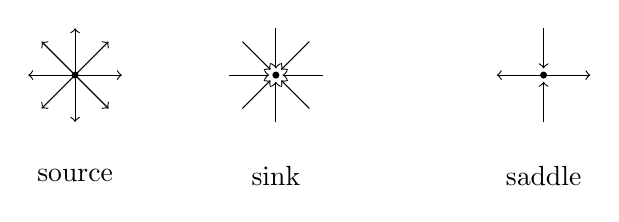
\begin{tikzpicture}[scale=0.85]
    % Source
    \node at (0,-1.5) {source};
    \fill (0,0) circle (1.5pt);
    \draw[->] (0,0) -- (0.7,0);
    \draw[->] (0,0) -- (-0.7,0);
    \draw[->] (0,0) -- (0,0.7);
    \draw[->] (0,0) -- (0,-0.7);
    \draw[->] (0,0) -- (0.5,0.5);
    \draw[->] (0,0) -- (-0.5,0.5);
    \draw[->] (0,0) -- (0.5,-0.5);
    \draw[->] (0,0) -- (-0.5,-0.5);
    % Sink
    \begin{scope}[xshift=3cm]
        \node at (0,-1.5) {sink};
        \fill (0,0) circle (1.5pt);
        \draw[->] (0.7,0) -- (0.1,0);
        \draw[->] (-0.7,0) -- (-0.1,0);
        \draw[->] (0,0.7) -- (0,0.1);
        \draw[->] (0,-0.7) -- (0,-0.1);
        \draw[->] (0.5,0.5) -- (0.08,0.08);
        \draw[->] (-0.5,0.5) -- (-0.08,0.08);
        \draw[->] (0.5,-0.5) -- (0.08,-0.08);
        \draw[->] (-0.5,-0.5) -- (-0.08,-0.08);
    \end{scope}
    % Saddle
    \begin{scope}[xshift=7cm]
        \node at (0,-1.5) {saddle};
        \fill (0,0) circle (1.5pt);
        % In along y, out along x
        \draw[->] (0,0.7) -- (0,0.1);
        \draw[->] (0,-0.7) -- (0,-0.1);
        \draw[->] (0,0) -- (0.7,0);
        \draw[->] (0,0) -- (-0.7,0);
    \end{scope}
\end{tikzpicture}
\end{center}

\subsection{Euler Characteristic from Local Lefschetz Numbers}

\begin{example}{Euler Characteristic of $S^2$}{euler-S2-downward-flow}
    Consider the map $f_t \colon S^2 \to S^2$ given by a ``downward flow''
    \[
        f_t(x) = \pi\!\left(x + \left(0, 0, -\tfrac{t}{2}\right)\right), \quad 0 < t < 2,
    \]
    where $\pi \colon \R^3 \setminus \{0\} \to S^2$ is the projection. This has a source at the north pole and a sink at the south pole, giving
    \[
        \chi(S^2) = L(f_1) = 1 + 1 = 2.
    \]
\end{example}

\begin{center}
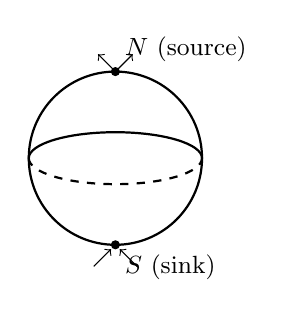
\begin{tikzpicture}[scale=1.1]
    % Sphere
    \draw[thick] (0,0) circle (1);
    \draw[thick,dashed] (-1,0) arc(180:360:1 and 0.3);
    \draw[thick] (-1,0) arc(180:0:1 and 0.3);
    % North pole (source)
    \fill (0,1) circle (1.5pt);
    \node[above right] at (0,1) {\small $N$ (source)};
    \draw[->] (0,1) -- (0.2,1.2);
    \draw[->] (0,1) -- (-0.2,1.2);
    % South pole (sink)
    \fill (0,-1) circle (1.5pt);
    \node[below right] at (0,-1) {\small $S$ (sink)};
    \draw[->] (0.25,-1.25) -- (0.05,-1.05);
    \draw[->] (-0.25,-1.25) -- (-0.05,-1.05);
\end{tikzpicture}
\end{center}

\begin{corollary}{Fixed Points of Maps on $S^2$}{s2-fixed-point}
    Every map $f \colon S^2 \to S^2$ homotopic to the identity must have a fixed point. In particular, the antipodal map $x \mapsto -x$ is not homotopic to the identity.
\end{corollary}

More generally, a genus $g$ surface admits a Lefschetz map homotopic to the identity that has $1$ source, $1$ sink, and $2g$ saddles, giving
\[
    \chi(\Sigma_g) = 2 - 2g.
\]

It is also instructive to see how the fixed points get created and annihilated in pairs when we deform the ``height function''; for example, on $S^2$,
\[
    \chi(S^2) = 1 + 1 = 1 + 1 + (1 - 1).
\]
